\documentclass[theme = fancy, zihao = 5]{work-template}
\wktempset{
    style = {
        font = times,
        cjk-font = sourcehan,
        today = big,                                   % 大写日期
        enname,                                        % 英文标题
        punct = CCT,
        fullwidth-stop                                 % 英文全角句点
    }
}
\title{\textsf{work-template}模板测试}
\author{Evistix}
\date{\today}

\usepackage{zhlipsum,lipsum}

\begin{document}
\maketitle

\part{段落测试}
\section{正文}
你好,\LaTeX!\par
句号测试1。句号测试2.\par
114514.

\part{数学测试}
\section{高斯定理}

数学字体:
\begin{equation}
    \int_V \nabla\times \symbf F\,\mathrm{d}V = \int_{\partial V} \symbf F\cdot\mathrm{d}\symbf S 
\end{equation}

\part{\LaTeX3 语法学习}
\section{TikZ测试}

\subsection{Right Triangle}
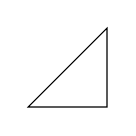
\begin{tikzpicture}
    \draw (0,0) -- (1,0) -- (1,1) -- cycle;
\end{tikzpicture}

\subsection{圆的参数方程}
$\begin{cases}
    x = r \cos\theta \\
    y = r \sin\theta  
\end{cases}$
$\left\{
    \begin{aligned}
        x = r \cos\theta \\
        y = r \sin\theta 
    \end{aligned}\right.$
\ExplSyntaxOn
\begin{tikzpicture}
\int_step_inline:nnn { 0 } { 34 }
  {
    \fp_set:Nn \l_tmpa_fp { 10 * (#1) * \c_one_degree_fp }
    \node[minimum ~ width = 1.5mm, fill = red, draw = none, circle, inner ~ sep = 0pt] at 
    ( \fp_eval:n {cos(\l_tmpa_fp)},
      \fp_eval:n {sin(\l_tmpa_fp)}) {};
  }    
\end{tikzpicture}
\ExplSyntaxOff

\section{\LaTeX3 语法测试}
\subsection{函数测试}
\verb|\cs_meaning:N \g_tmpa_tl| 
\ExplSyntaxOn
\tl_gclear:N \g_tmpa_tl
\tl_gset:Nn \g_tmpa_tl { test }
\cs_meaning:N \g_tmpa_tl
\ExplSyntaxOff

\subsection{正割函数值表}
\ExplSyntaxOn
\seq_gclear:N \g_tmpa_seq 
\int_step_inline:nnn { 0 } { 8 } 
  {
    \seq_put_right:Nn \l_tmpa_seq
      {
        $\sec #1^\circ = \fp_eval:n { sec (#1 * \c_one_degree_fp)}$
      }
    \int_compare:nNnT { #1 } > { 0 }
      {
        \int_compare:nNnT { \int_mod:nn { #1 + 1 } { 3 } } = { 0 }
          {
            \seq_gput_right:Nx \g_tmpa_seq 
              { \seq_use:Nn \l_tmpa_seq { & } }
            \seq_clear:N \l_tmpa_seq
          }
      }
  }
\ExplSyntaxOff
\ExplSyntaxOn
\seq_gclear:N \g_tmpb_seq 
\int_step_inline:nnn { 0 } { 2 } 
  {
    \seq_put_right:Nn \l_tmpa_seq
      {
        $\sin #1^\circ = \fp_eval:n { sin (#1 * \c_one_degree_fp)}$
      }
    \int_compare:nNnT { #1 } > { 0 }
      {
        \int_compare:nNnT { \int_mod:nn { #1 + 1 } { 3 } } = { 0 }
          {
            \seq_gput_right:Nx \g_tmpa_seq 
              { \seq_use:Nn \l_tmpa_seq { & } }
            \seq_clear:N \l_tmpa_seq
          }
      }
  }
\ExplSyntaxOff

\ExplSyntaxOn
%\tiny
\centering
\begin{tabular}{lll}
    \hline
    \seq_use:Nn \g_tmpa_seq { \\ }

    \seq_use:Nn \g_tmpb_seq { \\ }
    \\ \hline
\end{tabular}
\ExplSyntaxOff


\subsection{循环语句}
\ExplSyntaxOn
\int_step_inline:nn { 3 } 
  {
    \int_step_inline:nn { 3 }
      {
        \int_step_inline:nn { 3 }
          { (#1,##1,####1),~ }
      }
  }
\ExplSyntaxOff
\end{document}